% Szglab4
% ===========================================================================
%
\chapter{Analízis modell kidolgozása 1}

\thispagestyle{fancy}

\section{Objektum katalógus}

\subsection{Command}
\begin{tabularx}{\linewidth}{| l | X |}
\hline
\textbf{Név} & \textbf{Leírás} \tabularnewline
\hline\hline
\endhead
ChangeDirectionQuery & Egy robottól irányváltoztatást kérő parancs. Elő tudja állítani a megfelelő \textbf{ChangeDirectionTransmit} parancsot. \tabularnewline\hline

ChangeDirectionTransmit & Az az irányváltoztató parancs, amit egy cella módosítani tud a rajta található buffokkal. Elő tudja állítani a megfelelő \textbf{ChangeDirectionExecute} parancsot. \tabularnewline\hline 

ChangeDirectionExecute & Az ugrást a \textbf{Roboton} ténylegesen végrehajtó parancs. \tabularnewline\hline

ChangeSpeedQuery & Egy robottól sebességváltoztatást kérő parancs. Elő tudja állítani a megfelelő \textbf{ChangeSpeedTransmit} parancsot. \tabularnewline\hline

ChangeSpeedTransmit & Az a sebességváltoztató parancs, amit egy cella módosítani tud a rajta található buffokkal. Elő tudja állítani a megfelelő \textbf{ChangeSpeedExecute} parancsot. \tabularnewline\hline

ChangeSpeedExecute & A sebességváltoztatást a \textbf{Roboton} ténylegesen végrehajtó parancs. \tabularnewline\hline

JumpQuery & Egy robottól ugrás kezdeményezését kérő parancs. Lekérdezi és tárolja a robot aktuális sebességét. Elő tudja állítani a megfelelő \textbf{JumpTransmit} parancsot.  \tabularnewline\hline

JumpTransmit & Az az ugróparancs, amit egy cella módosítani tud a rajta található buffokkal. Lekérdezi a cellától az ugrás kezdetét és célját, és tárolja ezeket. Elő tudja állítani a megfelelő \textbf{JumpExecute} parancsot. \tabularnewline\hline 

JumpExecute & Az ugrást a \textbf{Roboton}, a kezdő és cél cellán ténylegesen végrehajtó parancs. \tabularnewline\hline

KillExecute & Egy \textbf{Robotot} a játékból kiiktatni képes parancs. \tabularnewline\hline

TimoutExecute & Egy \textbf{Robotnak} jelzi, hogy elfogyott a rá kijelölt teljes időtartam. \tabularnewline\hline

UseOilQuery & Egy \textbf{Robotot} arra utasít, hogy helyezzen egy \textbf{Oil} buffot arra a mezőre, amelyen áll. Lekérdezi, hogy a robotnak van-e elérhető \textbf{Oil} készlete, és ezt tárolja. Elő tudja állítani a megfelelő \textbf{UseOilExecute} parancsot. \tabularnewline\hline

UseOilExecute & Egy \textbf{Oil} buffot helyez el a cellán. \tabularnewline\hline

UseStickyQuery & Egy \textbf{Robotot} arra utasít, hogy helyezzen egy \textbf{Sticky} buffot arra a mezőre, amelyen áll. Lekérdezi, hogy a robotnak van-e elérhető \textbf{Sticky} készlete, és ezt tárolja. Elő tudja állítani a megfelelő \textbf{UseStickyExecute} parancsot. \tabularnewline\hline

UseStickyExecute & Egy \textbf{Sticky} buffot helyez el a cellán. \tabularnewline\hline
\end{tabularx}

\subsection{Direction}
Tárolja egy \textbf{Robot} lehetséges mozgási irányait, és egyben a megfelelő \textbf{Cellek} lehetséges szomszédossági viszonyait.

\subsection{EmptyFieldCell}
Az \textbf{EmptyFieldCell} osztály példányai a pálya azon részeit tárolja, amelyre lépve a \textbf{Robotok} kiesnek a játékból. Az ő felelőssége a robotnak elküldeni azt a parancsot, ami ezt a hatást előidézi (\textbf{KillExecute}).
Tárolja a rajta álló robotot, illetve referenciákat a szomszédos mezőkre, amiket a megfelelő \textbf{Direction} megadásával érhetünk el. Tartalmazza ezen felül a céltól való távolságot, amelyet a nyertes meghatározására használhatunk. Az ő felelőssége annak a cellának a megkeresése, amelyre egy \textbf{Robot} ugorhat. A cellán átmenő parancsokat módosíthatja a rajta található buffokkal.

\subsection{FieldCell}
Ezen osztály példányai alkotják a pálya legnagyobb részét: minden olyan cella, amely nem a célvonal része, illetve nem a pálya szélét alkotja ilyen típusú. A \textbf{FieldCell} példányok fontos feldata, hogy a rálépő \textbf{Robotokon} érvényesítse a cellán lévő buffokat. Ezen felül a \textbf{Robotoknak} érkező parancsok egy része keresztülhalad ezeken a mezőkön, ahol a rajta található buffok ezeket a parancsokat módosíthatják. A \textbf{FieldCell} ezután a módosított parancsot
továbbítja a rajta álló \textbf{Robot} felé.
Tárolja a rajta álló robotot, illetve referenciákat a szomszédos mezőkre, amiket a megfelelő \textbf{Direction} megadásával érhetünk el. Tartalmazza ezen felül a céltól való távolságot, amelyet a nyertes meghatározására használhatunk. Az ő felelőssége annak a cellának a megkeresése, amelyre egy \textbf{Robot} ugorhat. A cellán átmenő parancsokat módosíthatja a rajta található buffokkal.

\subsection{FinishLineFieldCell}
A \textbf{FinishLineFieldCell} osztály példányainak felelősségei megegyeznek a \textbf{FieldCell} osztály példányainak felelősségeivel, azzal a különbséggel, hogy ezek a cellák jelzik egy körnek a végét.

\subsection{Inventory}
Buffok tárolására alkalmas, nyílvántartja a benne található buffok számát, és csak akkor engedi azokat használni, ha legalább egyet tartalmaz.

\subsection{Oil}
Egy olyan buff, aminek hatására a \textbf{Fieldre} lépő \textbf{Robotok} sebessége megfelelződik.

\subsection{Result}
Egy parancs lefutásának eredményét tárolja.

\subsection{Robot}
A \textbf{Robot} osztály példányai egy-egy pályán mozgó robotot tárolnak. Tárolja a saját sebességét, illetve azt a cellát, amin pillanatnyilag áll. Ezen felül rendelkeznek \textbf{Inventorykkal}, amelyben \textbf{Stickyt} vagy \textbf{Oilt} tárolnak. Ezeket le tudják helyezni arra a cellára, amelyen állnak.

\subsection{Speed}
Egy \textbf{Robot} sebességét reprezentálja.

\subsection{Sticky}
Egy olyan buff, ami képes a \textbf{JumpExecute} parancs olyan módosítására, amely megakadályozza azt, hogy ez a parancs megváltoztassa egy \textbf{Robot} sebességét.


\begin{figure}[h]
\begin{center}
%\includegraphics[width=17cm]{chapters/chapter03/example.pdf}
\caption{x}
\label{fig:example1}
\end{center}
\end{figure}


\section{Osztályok leírása}
\comment{Az előző alfejezetben tárgyalt objektumok felelősségének formalizálása attribútumokká, metódusokká. Csak publikus metódusok szerepelhetnek. Ebben az alfejezetben megjelennek az interfészek, az öröklés, az absztrakt osztályok. Segédosztályokra még mindig nincs szükség. Az osztályok ABC sorrendben kövessék egymást. Interfészek esetén az Interfészek, Attribútumok pontok kimaradnak.}

\subsection{Osztály1}
\begin{itemize}
\item Felelősség\\
\comment{Mi az osztály felelőssége. Kb 1 bekezdés.}
\item Ősosztályok\\
\comment{Mely osztályokból származik (öröklési hierarchia)\newline
Legősebb osztály $\rightarrow$ Ősosztály2 $\rightarrow$ Ősosztály3...}
\item Interfészek\\
\comment{Mely interfészeket valósítja meg.}
\item Attribútumok\\
\comment{Milyen attribútumai vannak}
	\begin{itemize}
		\item attribútum1: attribútum jellemzése: mire való
		\item attribútum2: attribútum jellemzése: mire való
	\end{itemize}
\item Metódusok\\
\comment{Milyen publikus metódusokkal rendelkezik. Metódusonként egy-három mondat arról, hogy a metódus mit csinál.}
	\begin{itemize}
		\item int foo(Osztály3 o1, Osztály4 o2): metódus leírása
		\item int bar(Osztály5 o1): metódus leírása
	\end{itemize}
\end{itemize}

\subsection{Osztály2}
\begin{itemize}
\item Felelősség\\
\comment{Mi az osztály felelőssége. Kb 1 bekezdés.}
\item Ősosztályok\\
\comment{Mely osztályokból származik (öröklési hierarchia)\newline
Legősebb osztály $\rightarrow$ Ősosztály2 $\rightarrow$ Ősosztály3...}
\item Interfészek\\
\comment{Mely interfészeket valósítja meg.}
\item Attribútumok\\
\comment{Milyen attribútumai vannak}
	\begin{itemize}
		\item attribútum1: attribútum jellemzése: mire való
		\item attribútum2: attribútum jellemzése: mire való
	\end{itemize}
\item Metódusok\\
\comment{Milyen publikus metódusokkal rendelkezik. Metódusonként egy-három mondat arról, hogy a metódus mit csinál.}
	\begin{itemize}
		\item int foo(Osztály3 o1, Osztály4 o2): metódus leírása
		\item int bar(Osztály5 o1): metódus leírása
	\end{itemize}
\end{itemize}

\clearpage

\section{Statikus struktúra diagramok}

\begin{figure}[h]
\begin{center}
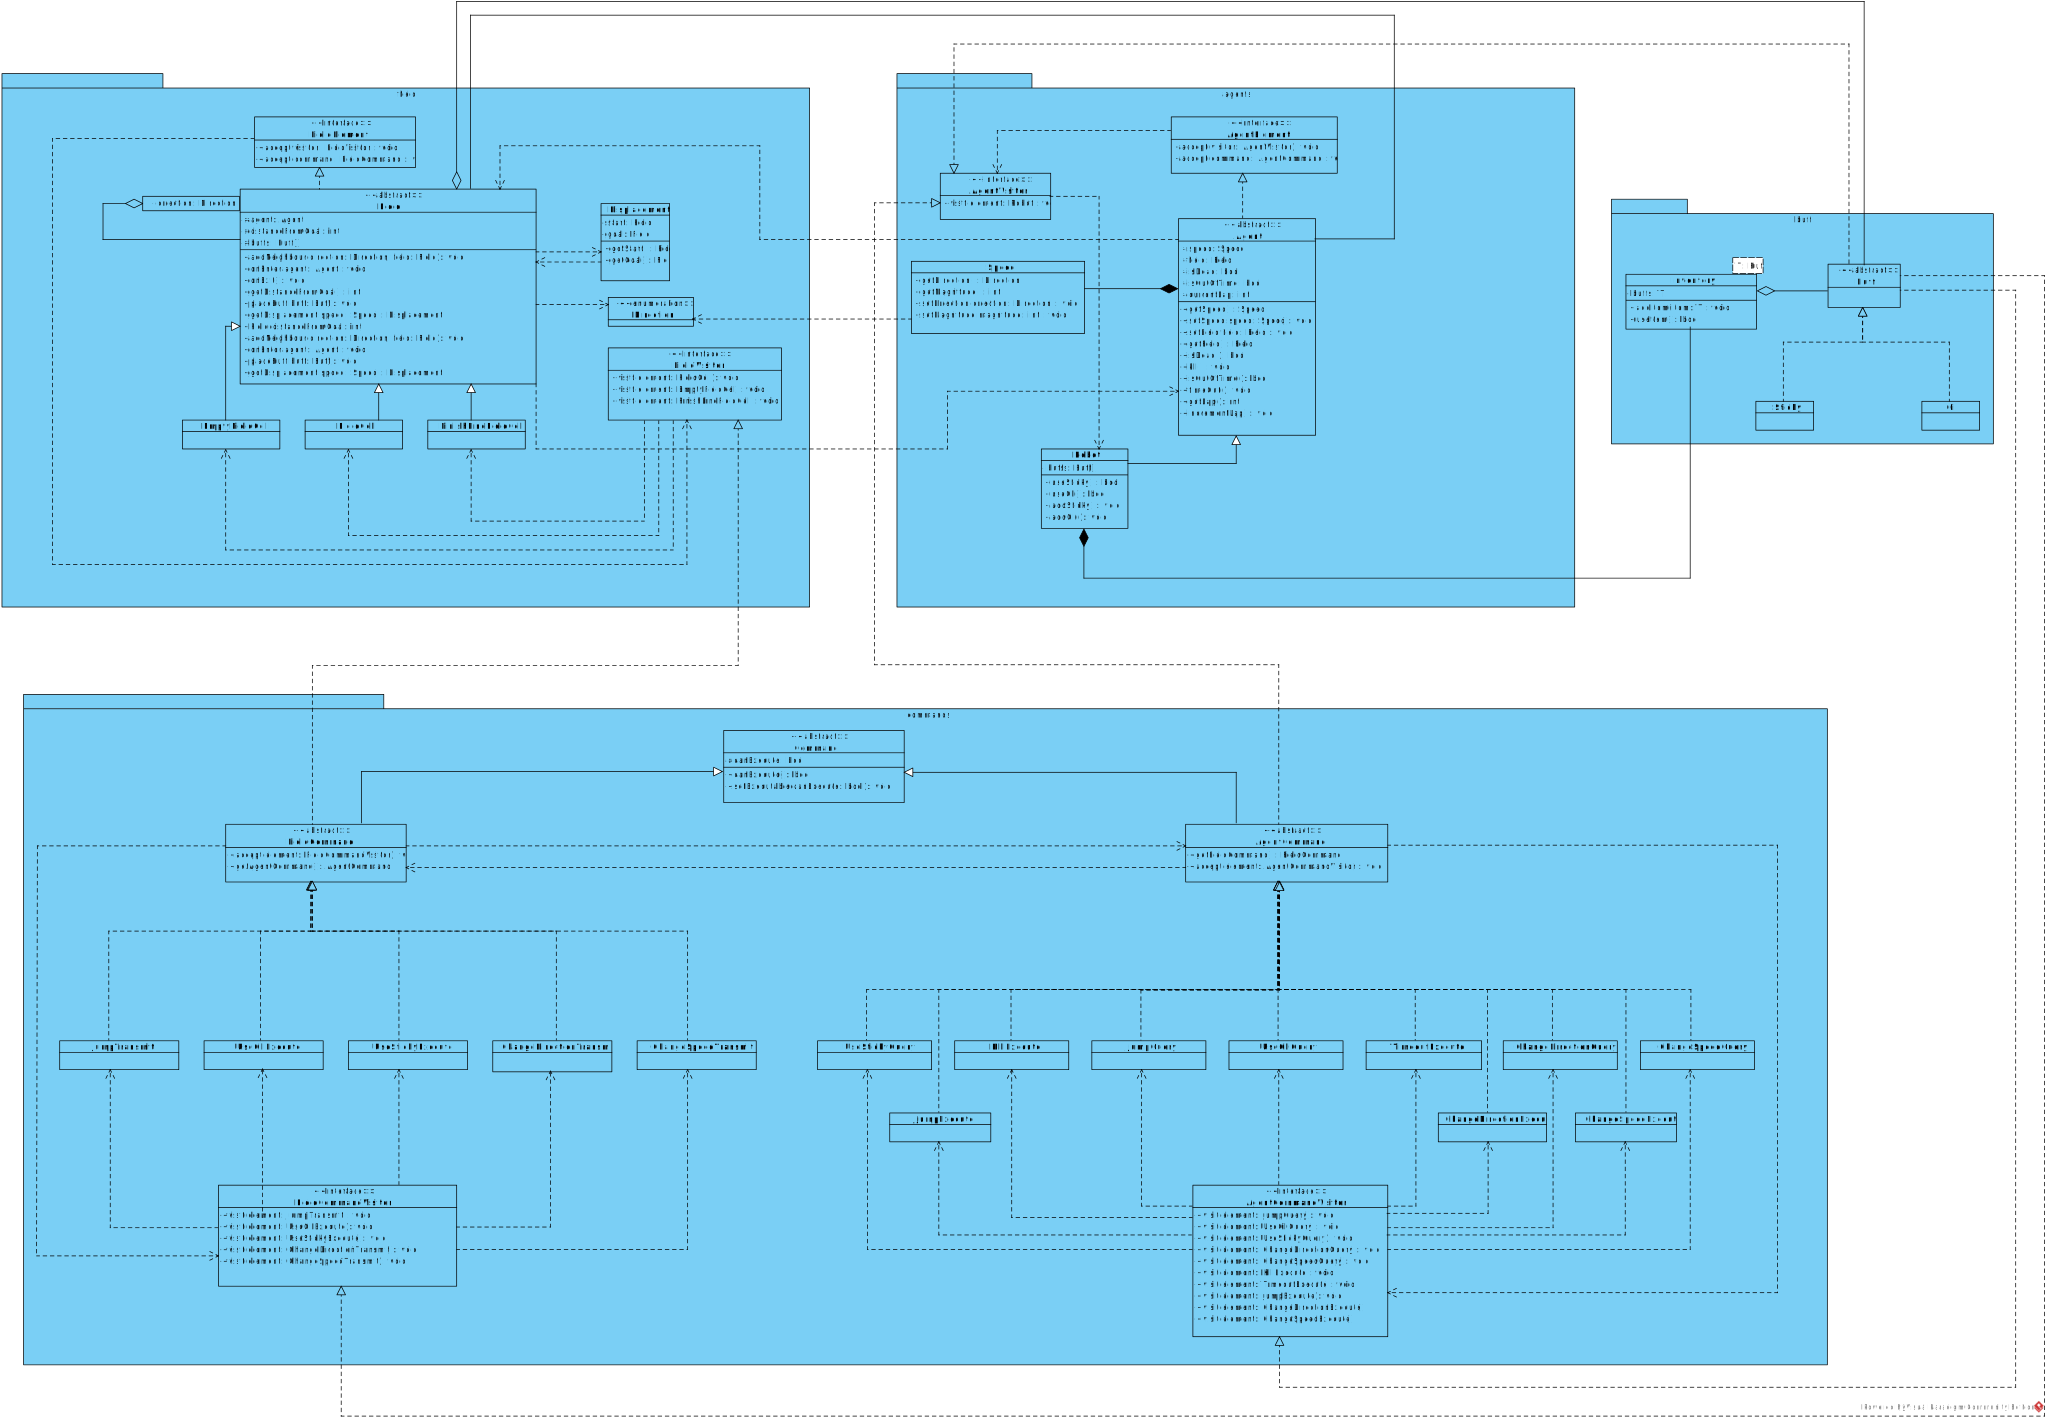
\includegraphics[width=\linewidth]{chapters/chapter03/ClassMain.pdf}
\caption{A teljes osztálydiagram}
\label{A teljes osztálydiagram}
\end{center}
\end{figure}

\begin{figure}[h]
\begin{center}
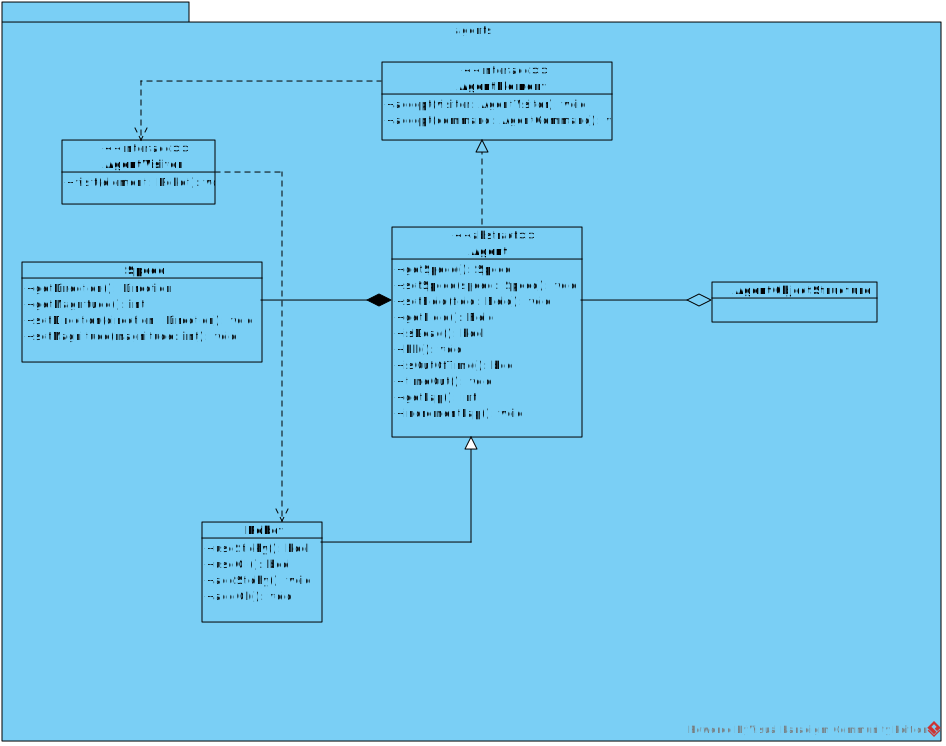
\includegraphics[width=\linewidth]{chapters/chapter03/ClassAgents.pdf}
\caption{Agents package osztálydiagram}
\label{Agents package osztálydiagram}
\end{center}
\end{figure}

\begin{figure}[h]
\begin{center}
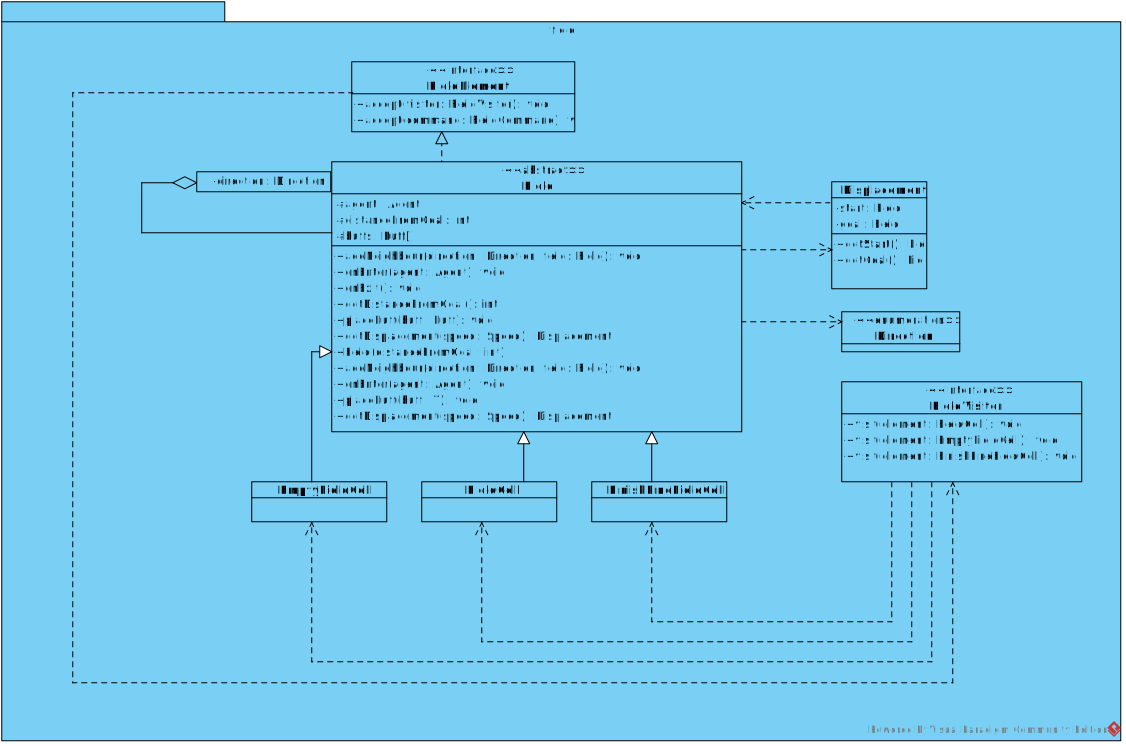
\includegraphics[width=\linewidth]{chapters/chapter03/ClassField.pdf}
\caption{Field package osztálydiagram}
\label{Field package osztálydiagram}
\end{center}
\end{figure}

\clearpage

\begin{figure}[h]
\begin{center}
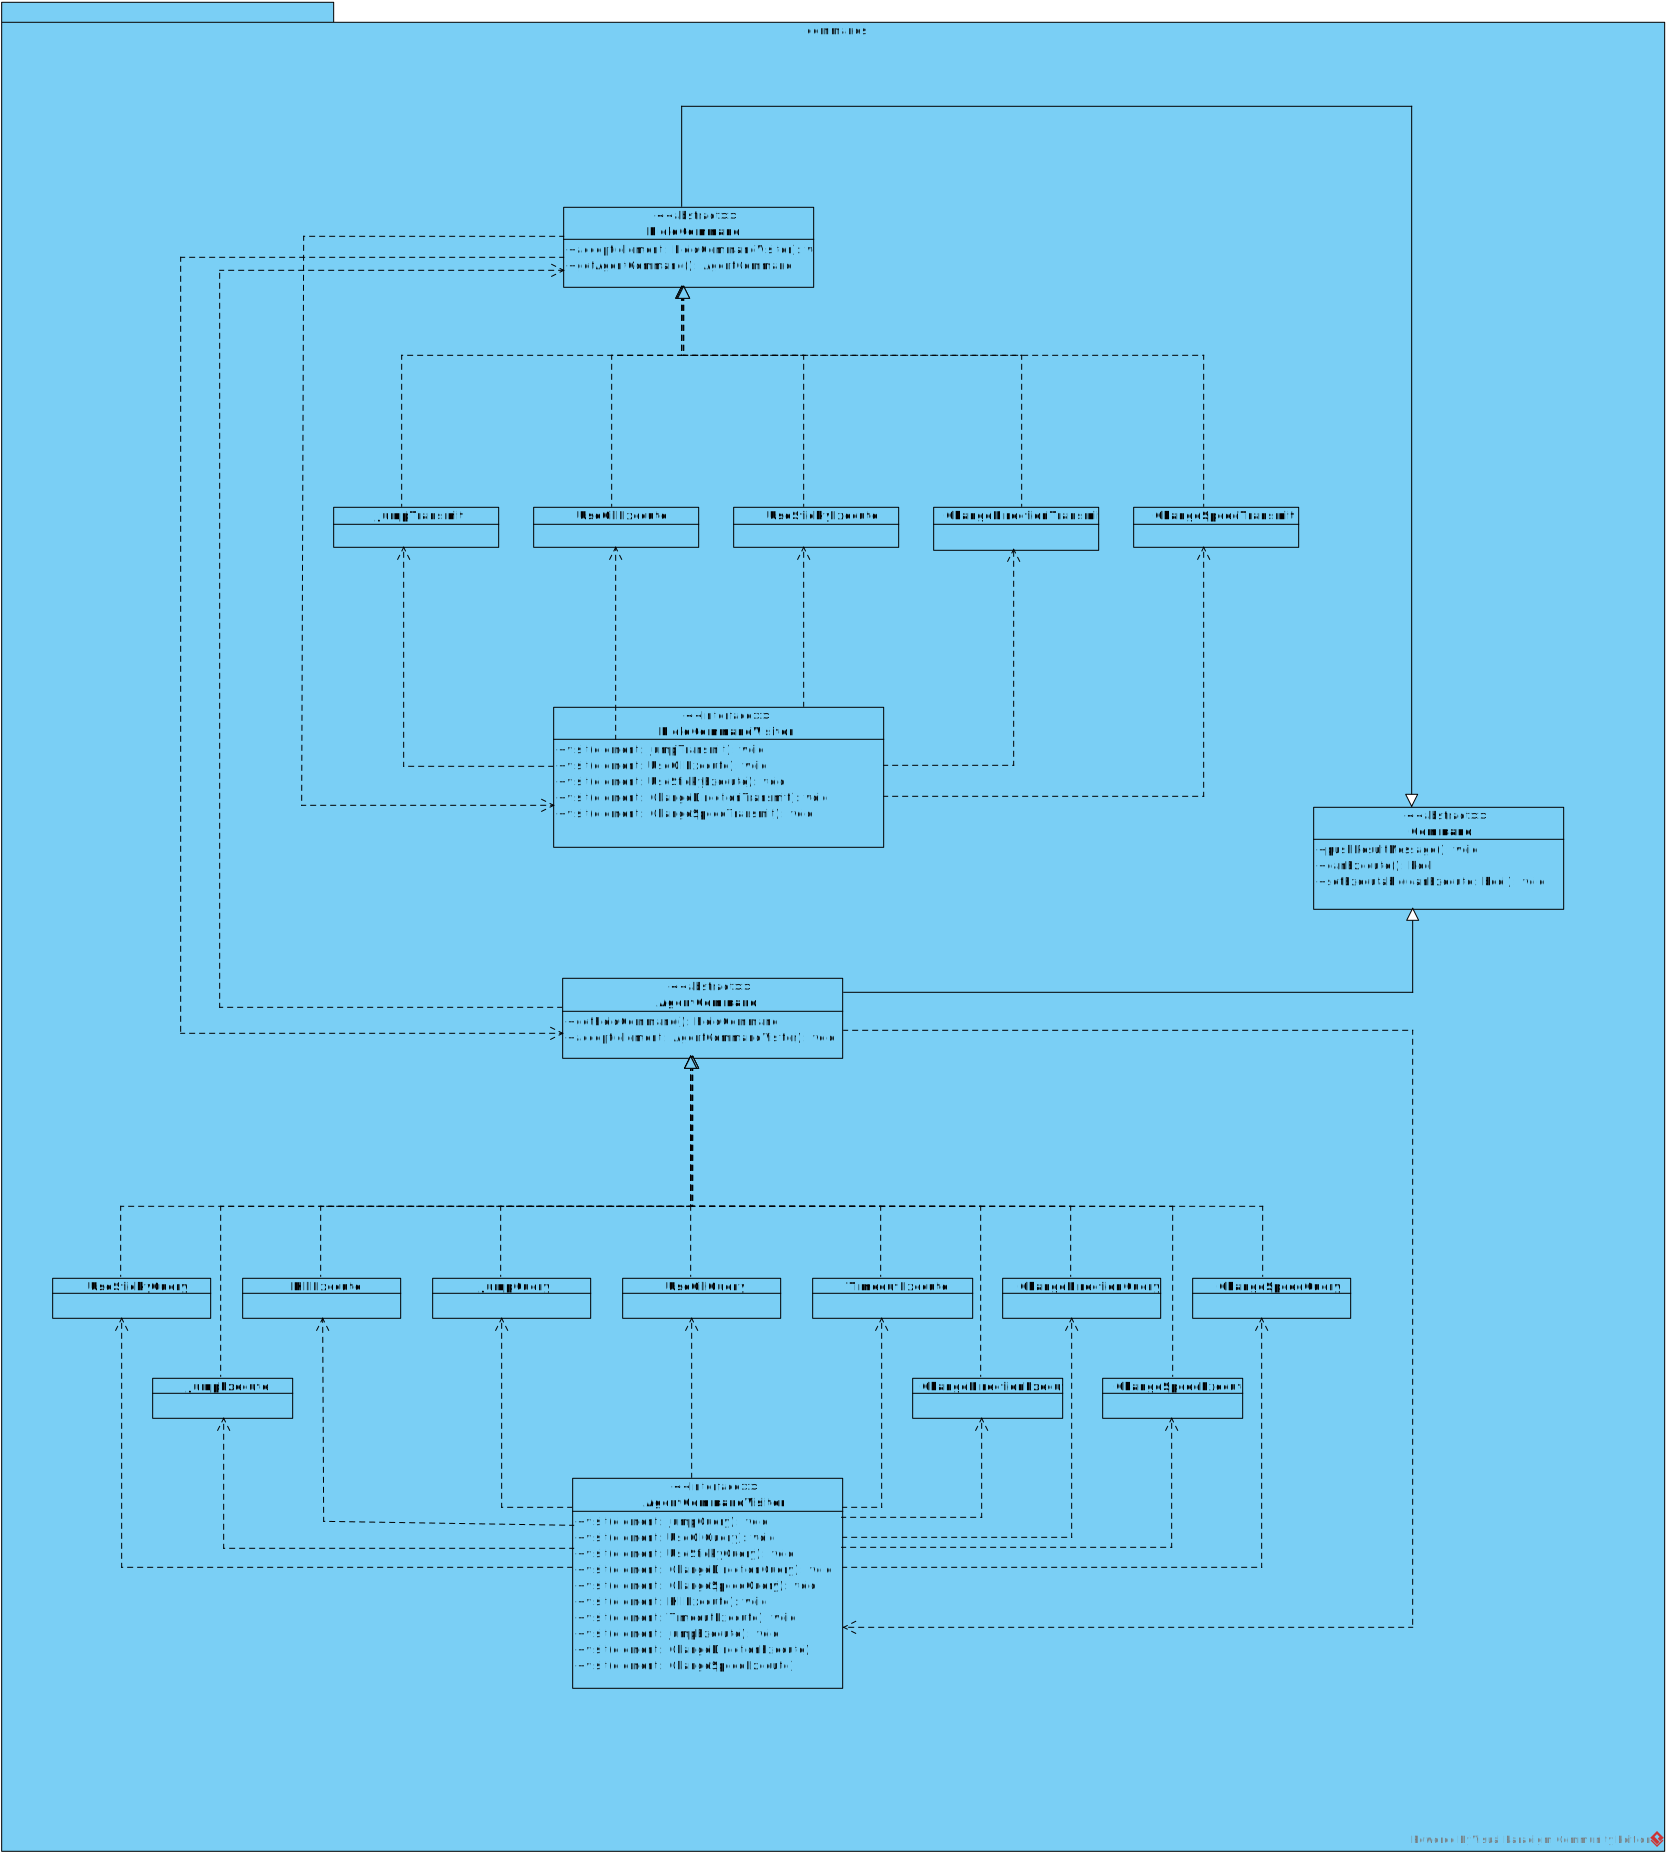
\includegraphics[width=\linewidth]{chapters/chapter03/ClassCommands.pdf}
\caption{Commands package osztálydiagram}
\label{Commands package osztálydiagram}
\end{center}
\end{figure}


\begin{figure}[h]
\begin{center}
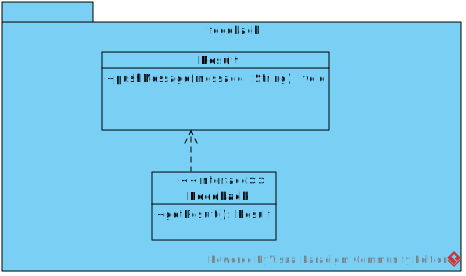
\includegraphics[width=\linewidth]{chapters/chapter03/ClassFeedback.pdf}
\caption{Feedback package osztálydiagram}
\label{Feedback package osztálydiagram}
\end{center}
\end{figure}


\begin{figure}[h]
\begin{center}
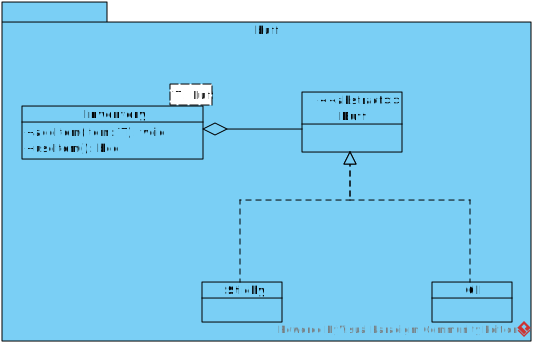
\includegraphics[width=\linewidth]{chapters/chapter03/ClassBuff.pdf}
\caption{Buff package osztálydiagram}
\label{Buff package osztálydiagram}
\end{center}
\end{figure}


\begin{figure}[h]
\begin{center}
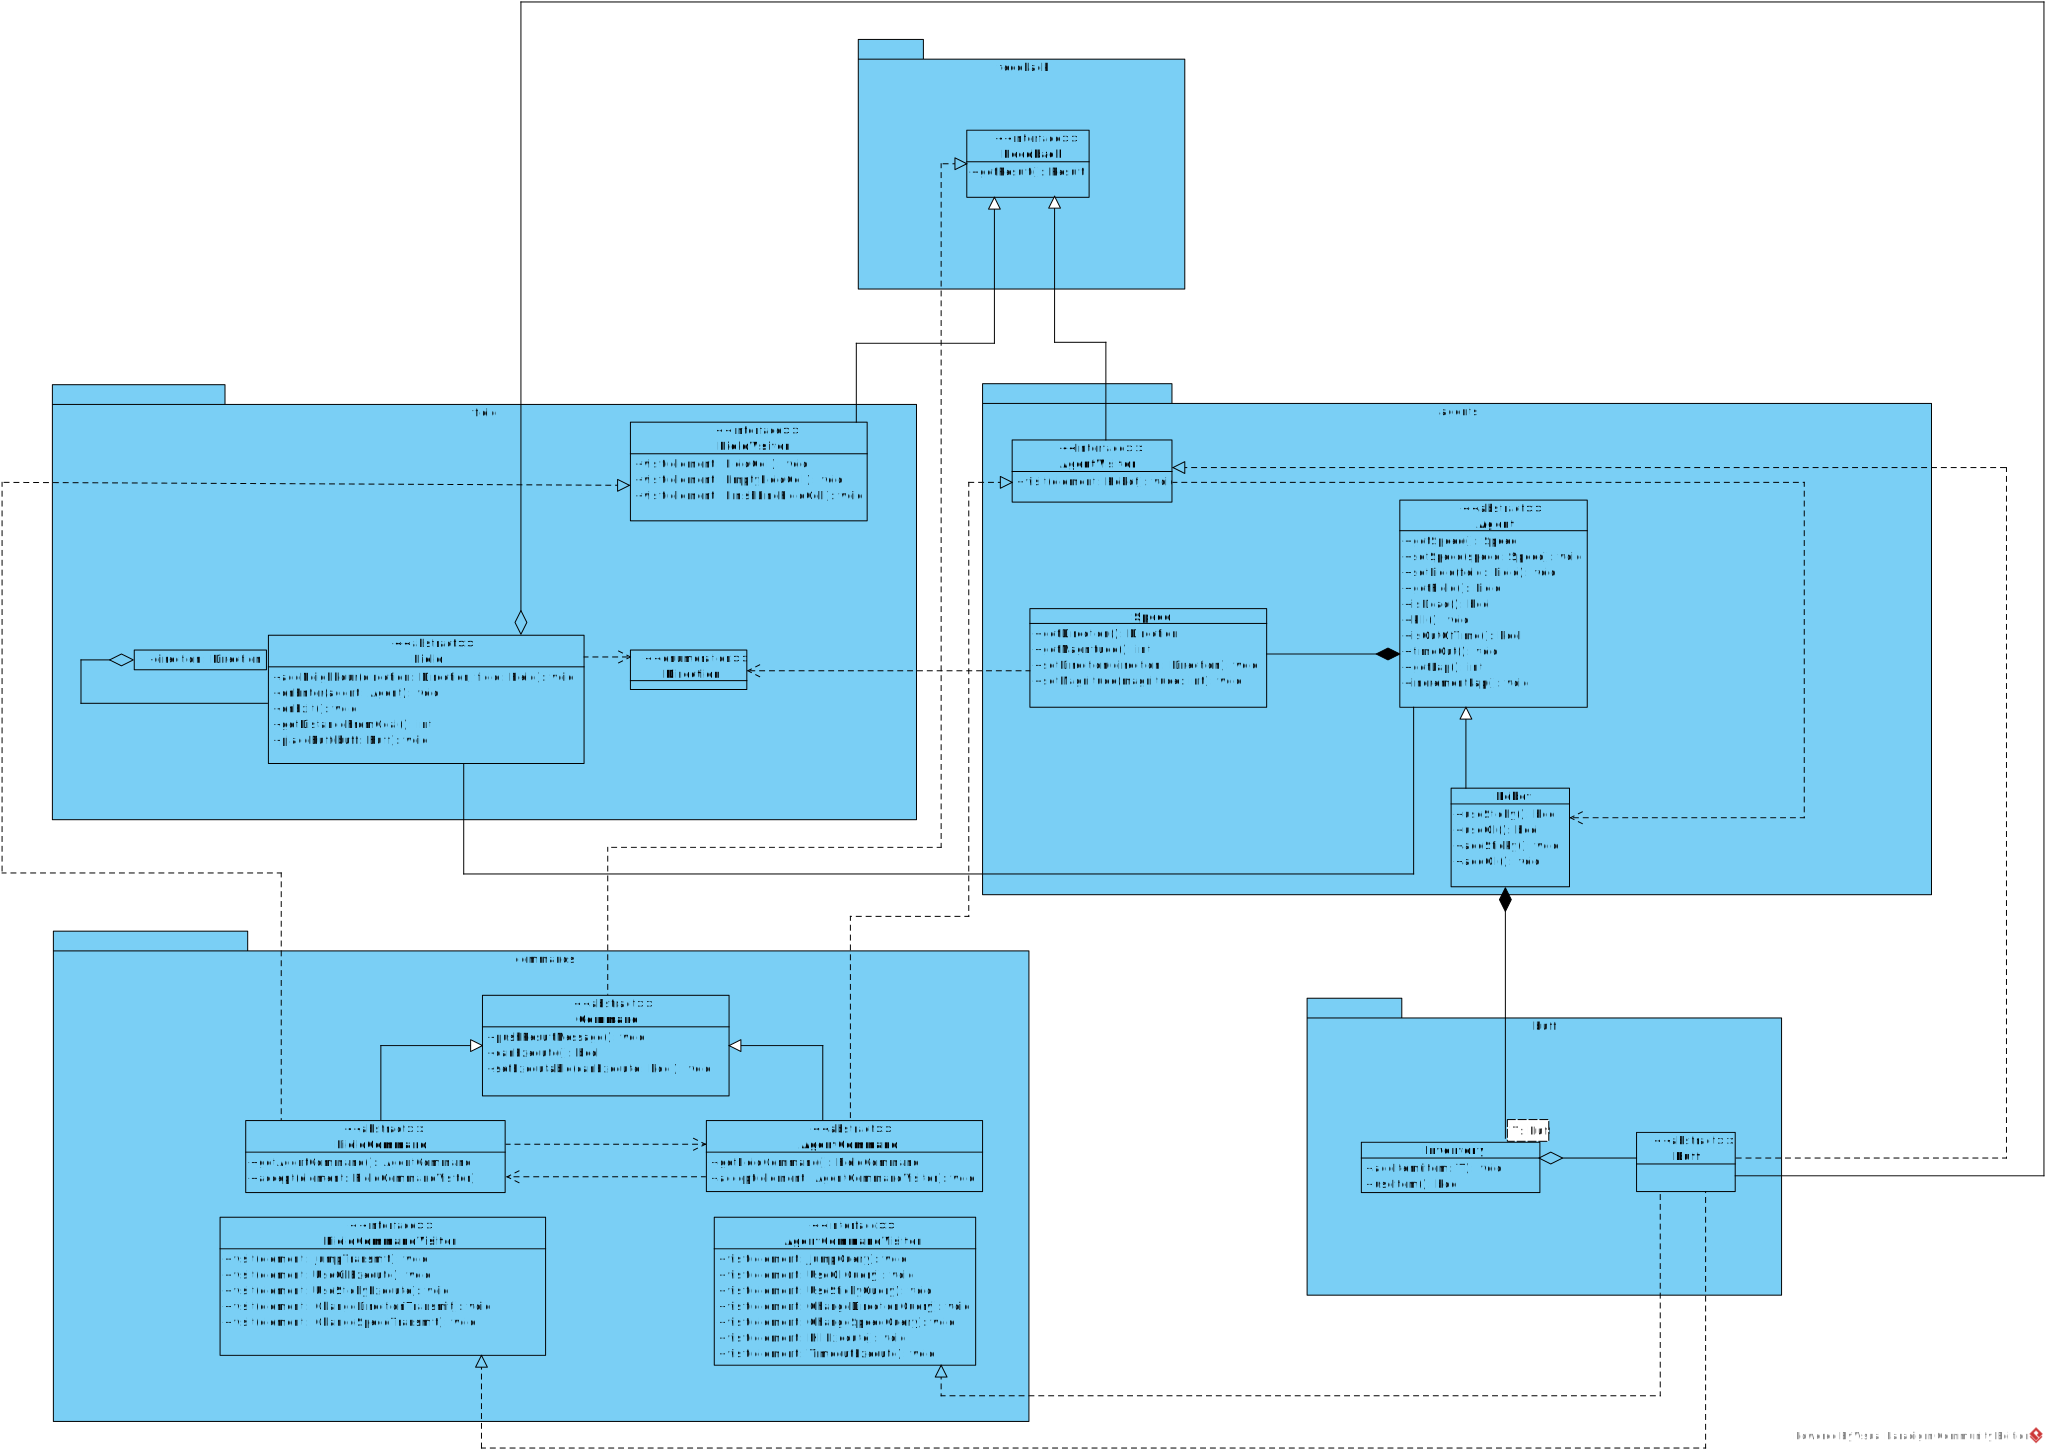
\includegraphics[width=\linewidth]{chapters/chapter03/ClassInterpackage.pdf}
\caption{Packagek közti függőségek osztálydiagramja}
\label{Packagek közti függőségek osztálydiagramja}
\end{center}
\end{figure}

\clearpage

\section{Szekvencia diagramok}

\begin{figure}[h]
	\begin{center}
		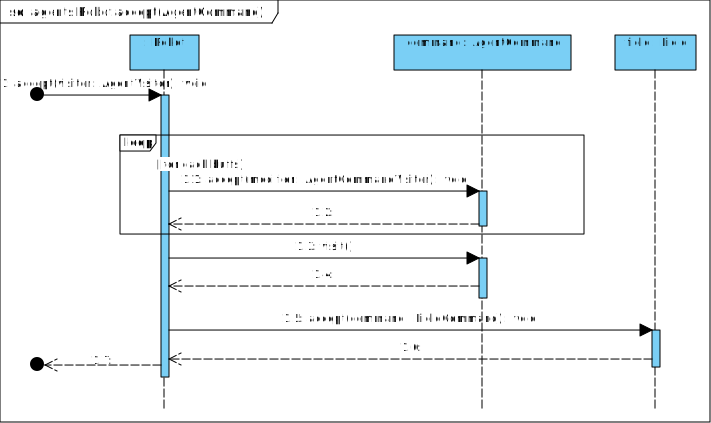
\includegraphics[width=\textwidth]{chapters/chapter03/agentsRobotacceptAgentCommand.pdf}
		\caption{Robot utasítást fogad}
		\label{fig:agents.Robot.accept}
	\end{center}
\end{figure}

\begin{figure}[h]
	\begin{center}
		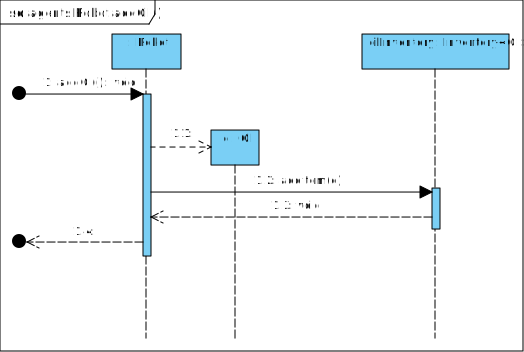
\includegraphics[width=\textwidth]{chapters/chapter03/agentsRobotaddOil.pdf}
		\caption{Robot felvesz a készletébe egy olajfoltot}
		\label{fig:agents.Robot.addOil}
	\end{center}
\end{figure}

\begin{figure}[h]
	\begin{center}
		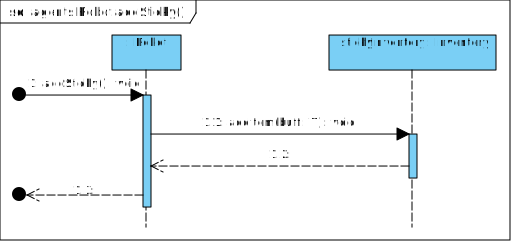
\includegraphics[width=\textwidth]{chapters/chapter03/agentsRobotaddSticky.pdf}
		\caption{Robot felvesz a készletébe egy ragacsfoltot}
		\label{fig:agents.Robot.addSticky}
	\end{center}
\end{figure}

\begin{figure}[h]
	\begin{center}
		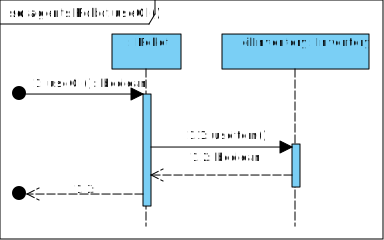
\includegraphics[width=\textwidth]{chapters/chapter03/agentsRobotuseOil.pdf}
		\caption{Robot felhasználja a készletében lévő olajfoltot ha van}
		\label{fig:agents.Robot.useOil}
	\end{center}
\end{figure}

\begin{figure}[h]
	\begin{center}
		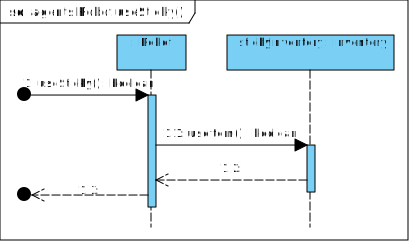
\includegraphics[width=\textwidth]{chapters/chapter03/agentsRobotuseSticky.pdf}
		\caption{Robot felhasználja a készletében lévő ragacsfoltot ha van}
		\label{fig:agents.Robot.useSticky}
	\end{center}
\end{figure}

\begin{figure}[h]
	\begin{center}
		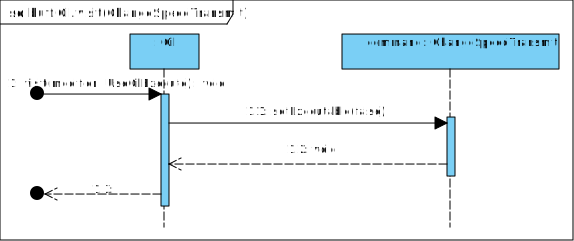
\includegraphics[width=\textwidth]{chapters/chapter03/buffOilvisitChangeSpeedTransmit.pdf}
		\caption{Olajfolt megakadályozza a sebesség nagyságának változtatását}
		\label{fig:buff.Oil.visit}
	\end{center}
\end{figure}

\begin{figure}[h]
	\begin{center}
		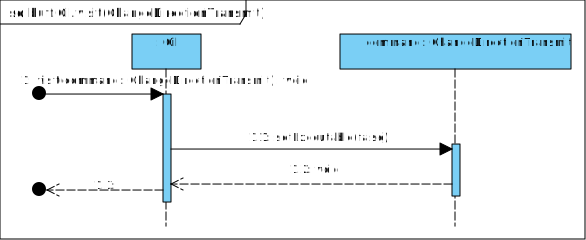
\includegraphics[width=\textwidth]{chapters/chapter03/buffOilvisitChangeDirectionTransmit.pdf}
		\caption{Olajfolt megakadályozza a sebesség irányának megváltoztatását}
		\label{fig:buff.Oil.visit2}
	\end{center}
\end{figure}

\begin{figure}[h]
	\begin{center}
		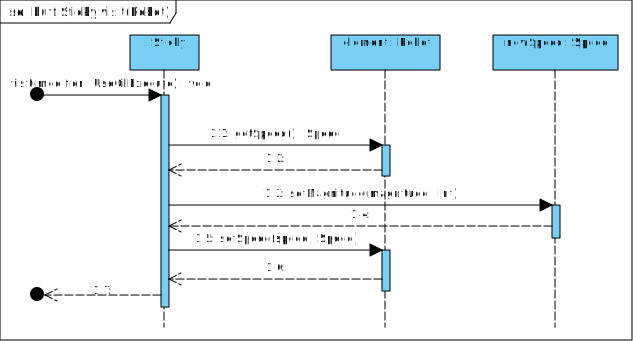
\includegraphics[width=\textwidth]{chapters/chapter03/buffStickyvisitRobot.pdf}
		\caption{Olajfolt megakadályozza a sebességváltoztatást}
		\label{fig:buff.Sticky.visit}
	\end{center}
\end{figure}

\begin{figure}[h]
	\begin{center}
		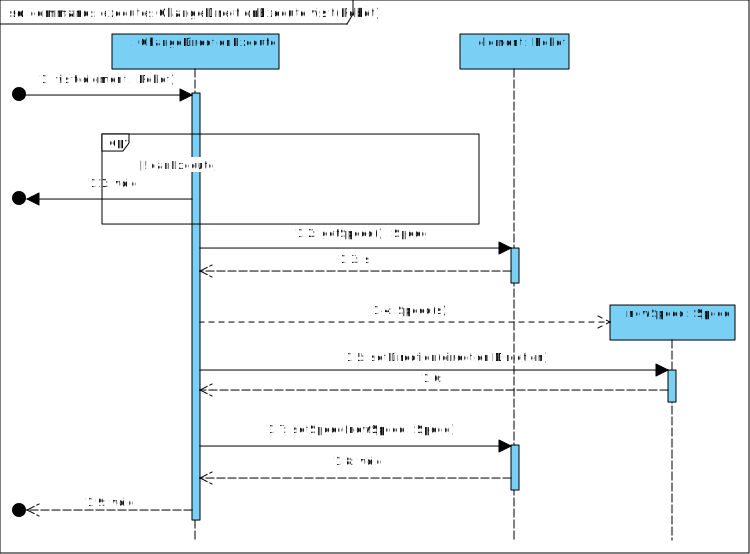
\includegraphics[width=\textwidth]{chapters/chapter03/commandsexecutesChangeDirectionExecutevisitRobot.pdf}
		\caption{Robot irányváltoztatásának végrehajtása}
		\label{fig:command.executes.ChangeDirectionExecute.visit}
	\end{center}
\end{figure}

\begin{figure}[h]
	\begin{center}
		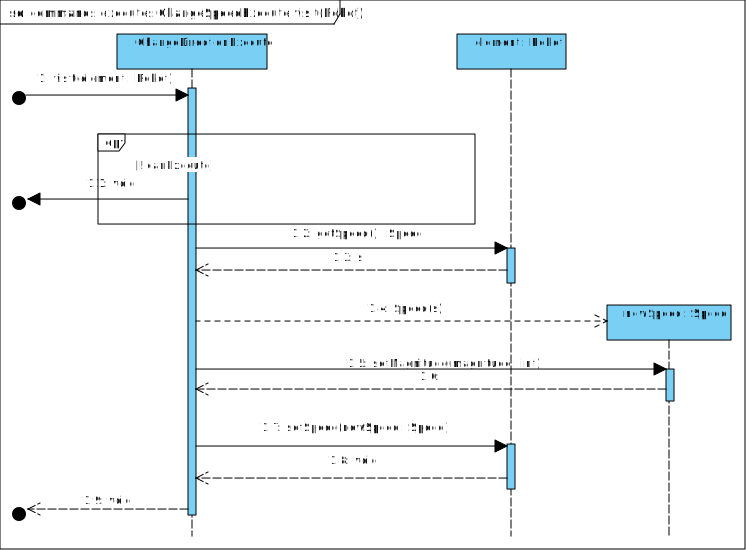
\includegraphics[width=\textwidth]{chapters/chapter03/commandsexecutesChangeSpeedExecutevisitRobot.pdf}
		\caption{Robot sebességnagyságának megváltoztatása}
		\label{fig:command.executes.ChangeSpeedExecute.visit}
	\end{center}
\end{figure}

\begin{figure}[h]
	\begin{center}
		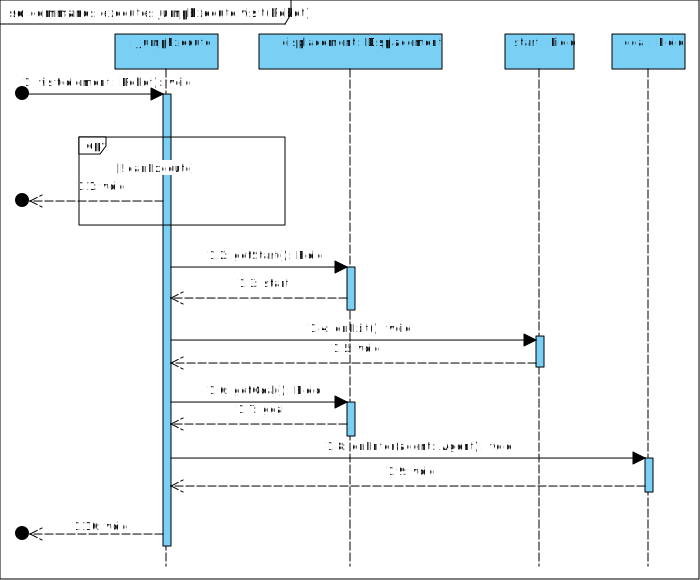
\includegraphics[width=\textwidth]{chapters/chapter03/commandsexecutesJumpExecutevisitRobot.pdf}
		\caption{Robot ugrásának végrehajtása}
		\label{fig:command.executes.JumpExecute.visit}
	\end{center}
\end{figure}

\begin{figure}[h]
	\begin{center}
		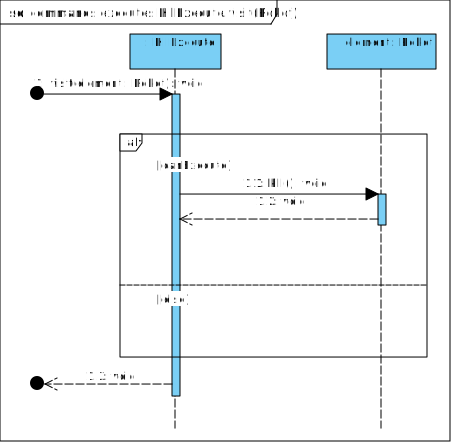
\includegraphics[width=\textwidth]{chapters/chapter03/commandsexecutesKillExecutevisitRobot.pdf}
		\caption{Robot megölésének végrehajtása}
		\label{fig:command.executes.KillExecute.visit}
	\end{center}
\end{figure}

\begin{figure}[h]
	\begin{center}
		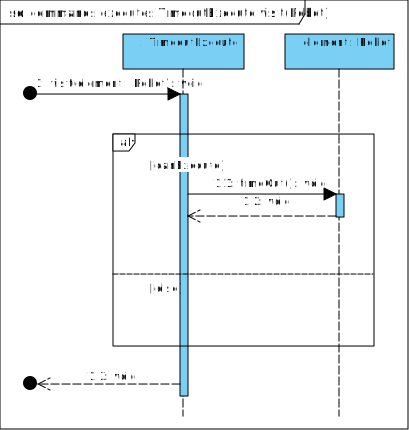
\includegraphics[width=\textwidth]{chapters/chapter03/commandsexecutesTimeoutExecutevisitRobot.pdf}
		\caption{Robot idő lejártának végrehajtása}
		\label{fig:command.executes.TimeoutExecute.visit}
	\end{center}
\end{figure}

\begin{figure}[h]
	\begin{center}
		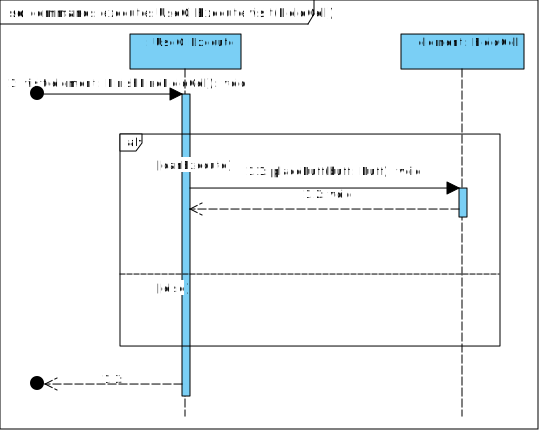
\includegraphics[width=\textwidth]{chapters/chapter03/commandsexecutesUseOilExecutevisitFieldCell.pdf}
		\caption{Robot lehelyezi az Olaj foltot a mezőre}
		\label{fig:command.executes.UseOilExecute.visit}
	\end{center}
\end{figure}

\begin{figure}[h]
	\begin{center}
		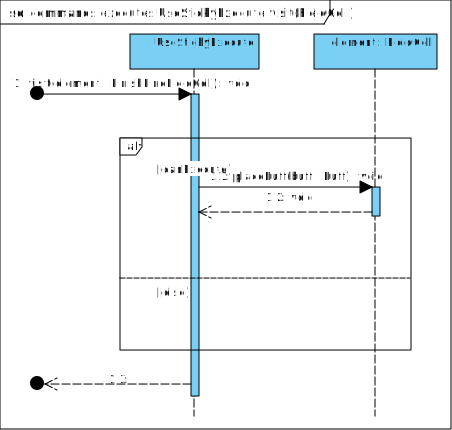
\includegraphics[width=\textwidth]{chapters/chapter03/commandsexecutesUseStickyExecutevisitFieldCell.pdf}
		\caption{Robot lehelyezi a Ragacs foltot a mezőre}
		\label{fig:command.executes.UseStickyExecute.visit}
	\end{center}
\end{figure}

\clearpage

\begin{figure}[h]
	\begin{center}
		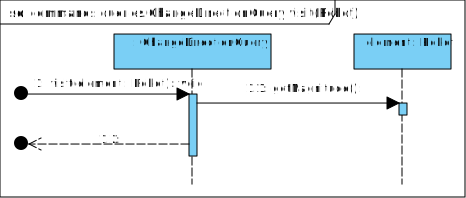
\includegraphics[width=\textwidth]{chapters/chapter03/commandsqueriesChangeDirectionQueryvisitRobot.pdf}
		\caption{Robot irányváltásra való felkérése}
		\label{fig:command.executes.ChangeDirectionQuery.visit}
	\end{center}
\end{figure}

\begin{figure}[h]
	\begin{center}
		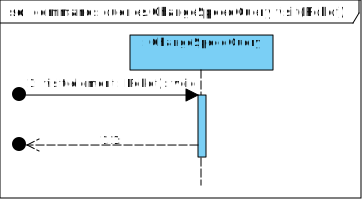
\includegraphics[width=\textwidth]{chapters/chapter03/commandsqueriesChangeSpeedQueryvisitRobot.pdf}
		\caption{Robot sebesség nagyságának megváltoztatására való felkérése}
		\label{fig:command.executes.ChangeSpeedQuery.visit}
	\end{center}
\end{figure}

\begin{figure}[h]
	\begin{center}
		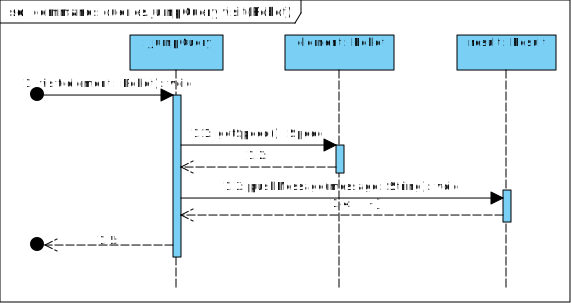
\includegraphics[width=\textwidth]{chapters/chapter03/commandsqueriesJumpQueryvisitRobot.pdf}
		\caption{Robot ugrásra azaz helyzetmódosításra való felkérése}
		\label{fig:command.executes.JumpQuery.visit}
	\end{center}
\end{figure}

\begin{figure}[h]
	\begin{center}
		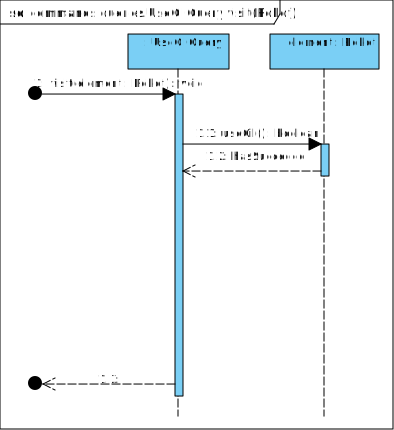
\includegraphics[width=\textwidth]{chapters/chapter03/commandsqueriesUseOilQueryvisitRobot.pdf}
		\caption{Robotot Olaj lehelyezésére való felkérése}
		\label{fig:command.executes.UseOilQuery.visit}
	\end{center}
\end{figure}

\begin{figure}[h]
	\begin{center}
		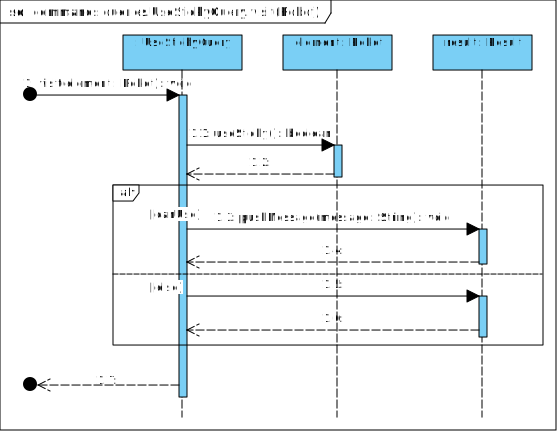
\includegraphics[width=\textwidth]{chapters/chapter03/commandsqueriesUseStickyQueryvisitRobot.pdf}
		\caption{Robotot Ragacs lehelyezésére való felkérése}
		\label{fig:command.executes.UseStickyQuery.visit}
	\end{center}
\end{figure}

\begin{figure}[h]
	\begin{center}
		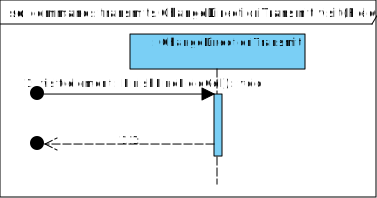
\includegraphics[width=\textwidth]{chapters/chapter03/commandstransmitsChangeDirectionTransmitvisitFieldCell.pdf}
		\caption{Irányváltásra vonatkozó kérés átvitele}
		\label{fig:command.executes.ChangeDirectionTransmit.visit}
	\end{center}
\end{figure}

\begin{figure}[h]
	\begin{center}
		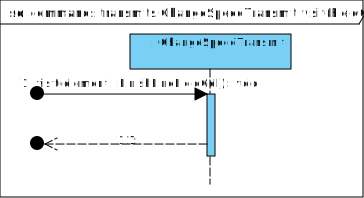
\includegraphics[width=\textwidth]{chapters/chapter03/commandstransmitsChangeSpeedTransmitvisitFieldCell.pdf}
		\caption{Szebességnagyság változtatásra vonatkozó kérés átvitele}
		\label{fig:command.executes.ChangeSpeedTransmit.visit}
	\end{center}
\end{figure}

\begin{figure}[h]
	\begin{center}
		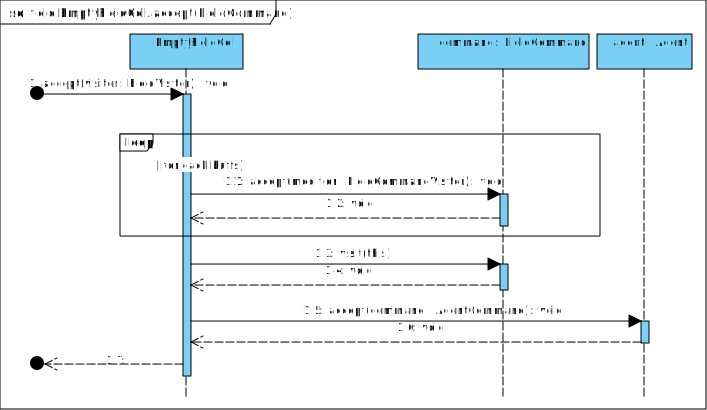
\includegraphics[width=\textwidth]{chapters/chapter03/fieldEmptyFieldCellacceptFieldCommand.pdf}
		\caption{Üres pályamező utasításfeldolgozása}
		\label{fig:field.EmptyFieldCell.accept}
	\end{center}
\end{figure}

\begin{figure}[h]
	\begin{center}
		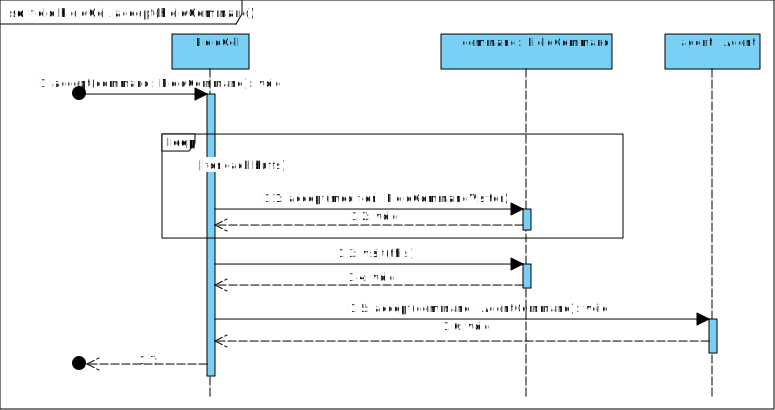
\includegraphics[width=\textwidth]{chapters/chapter03/fieldFieldCellacceptFieldCommand.pdf}
		\caption{Pályamező utasításfeldolgozása}
		\label{fig:field.FieldCell.accept}
	\end{center}
\end{figure}

\begin{figure}[h]
	\begin{center}
		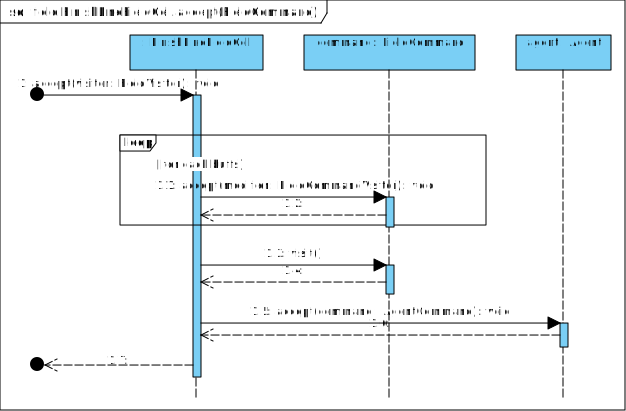
\includegraphics[width=\textwidth]{chapters/chapter03/fieldFinishLineFieldCellacceptFieldCommand.pdf}
		\caption{Start/célvonal pályamező utasításfeldolgozása}
		\label{fig:field.FinishLineFieldCell.accept}
	\end{center}
\end{figure}

\clearpage

\section{State-chartok}
\begin{figure}[h]
	\begin{center}
		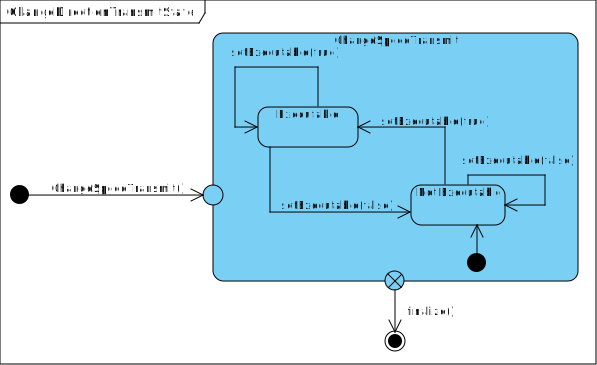
\includegraphics[width=\textwidth]{chapters/chapter03/ChangeDirectionTransmitState.pdf}
		\caption{ChangeDirectionTransmit osztály állapotdiagramja}
		\label{fig:state.ChangeDirectionTransmit}
	\end{center}
\end{figure}

\begin{figure}[h]
	\begin{center}
		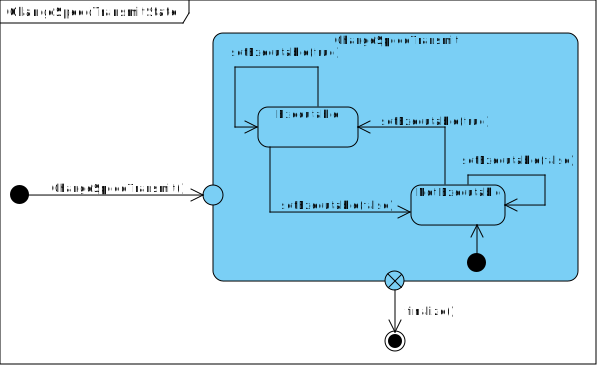
\includegraphics[width=\textwidth]{chapters/chapter03/ChangeSpeedTransmitState.pdf}
		\caption{ChangeSpeedTransmit osztály állapotdiagramja}
		\label{fig:state.ChangeSpeedTransmit}
	\end{center}
\end{figure}

\clearpage